\chapter{Deep Neural Networks}
\label{chapter:DNN}

This chapter introduces the concept of Deep Neural Networks (DNNs) and proceeds to Convolutional Neural Networks (CNNs), a common form of DNN widely used in image processing applications such as object detection. The evolution of CNNs and the associated popular models are further discussed. Field Programmable Gate Arrays (FPGAs) have recently been used to accelerate CNNs by developing dedicated hardware and memory systems. Thus, this chapter also focuses on the strategies implemented in previous works to accelerate CNNs in FPGAs.

%%%%%%%%%%%%%%%%%%%%%%%%%%%%%%%%%%%%%%%%%%%%%%%%%%%%%%%%%%%%%%%%%%%%%%%%
\section{Neural networks}
\label{section:NNs}

The neuron is the main computational unit of neural networks and is implemented as the weighted sum of the inputs plus a constant, followed by an activation function, as represented in Fig.~\ref{fig:neuron}.

\begin{figure}[!htb]
  \centering
  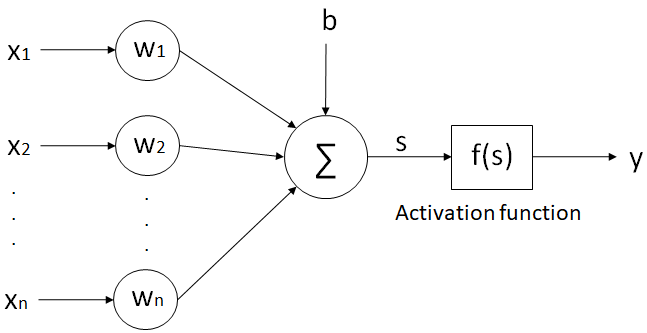
\includegraphics[width=0.45\textwidth]{Figures/neuron.png}
  \caption{Implementation of a neuron.}
  \label{fig:neuron}
\end{figure}
%\vspace{-2mm}

The weight, $w_{i}$, expresses the influence of a given input, $x_{i}$, to the neuron's output and the bias, $b$, is an offset term used to shift the result of the activation function, $f$, towards the negative or positive side. Eq. \ref{eq:NN} computes the output, $y$, of a neuron.

\begin{equation}
  y = f \left( b + \sum_{i=1}^{n} x_{i} w_{i} \right)
\label{eq:NN}
\end{equation}

Conventional activation functions include the identity function, the sigmoid (i.e., logistic function) and the hyperbolic tangent. Recently, the Rectified Linear Unit (ReLU) and some variations (e.g., Leaky ReLU) have become popular due to their simplicity and fast convergence during training~\cite{sze:dnn_survey}. These activation functions are represented in Fig.~\ref{fig:act_func}.    

\begin{figure}[!htb]
  \centering
  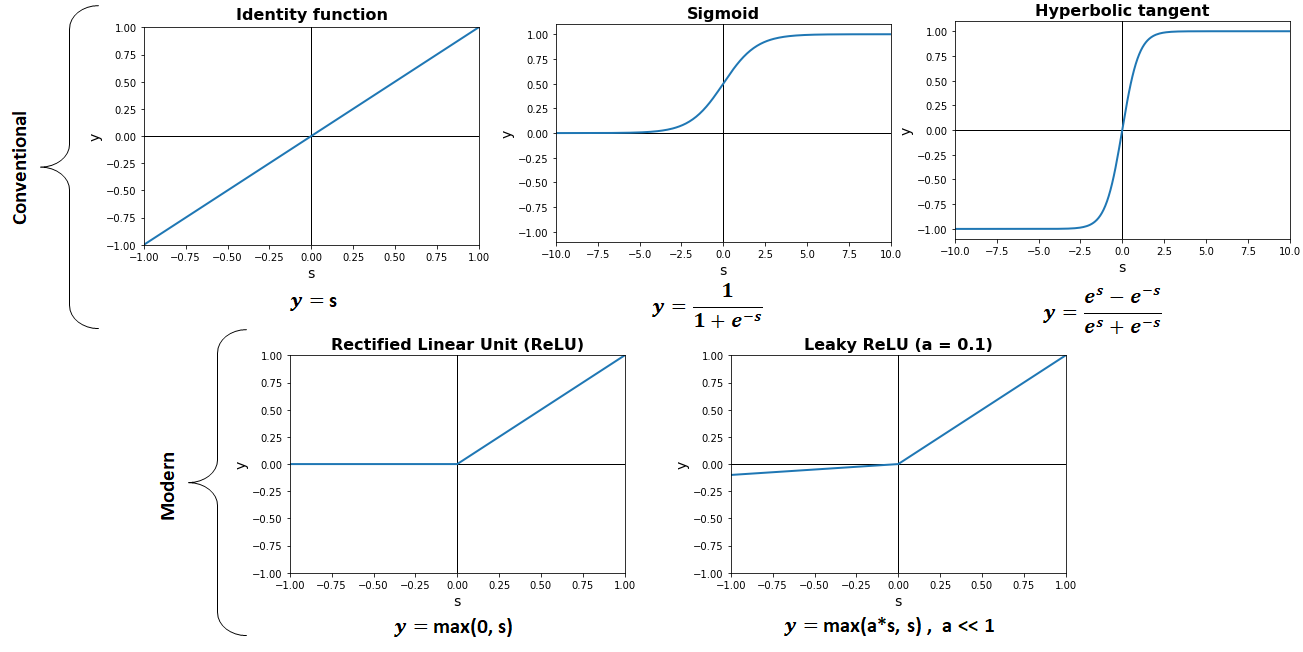
\includegraphics[width=\textwidth]{Figures/act_functions.png}
  \caption{Plot and expression of the most common activation functions.}
  \label{fig:act_func}
\end{figure}

Neural networks are composed by neurons organized in layers: one input layer, one or more hidden layers and one output layer. A DNN is a neural network with more than one hidden layer. Fig.~\ref{fig:DNN} exemplifies a fully connected (i.e., each neuron from one layer is connected to every neuron of the next layer) DNN with 2 hidden layers.

\vspace{-0.4cm}
\begin{figure}[!htb]
  \centering
  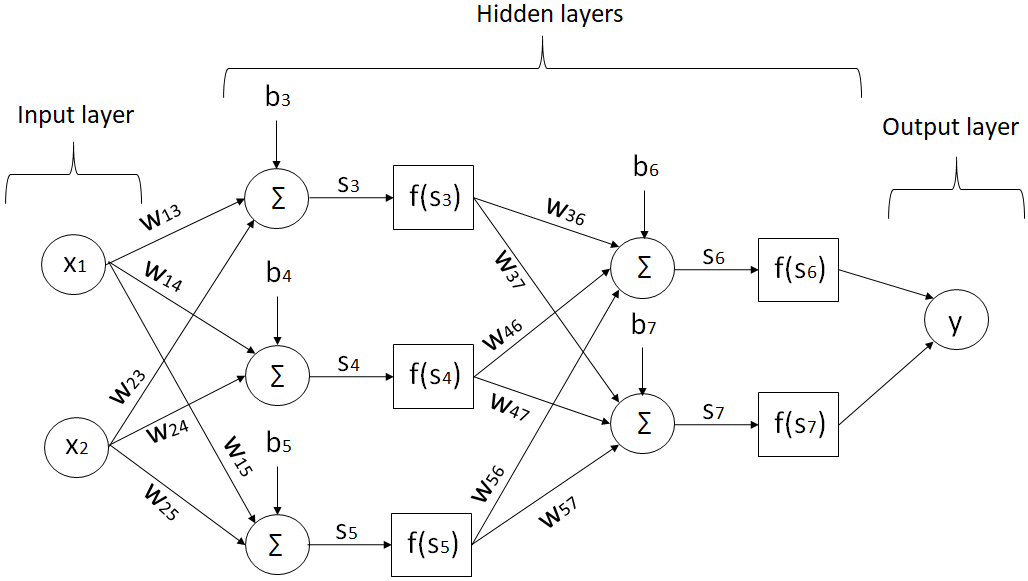
\includegraphics[width=0.7\textwidth]{Figures/DNN.png}
  \caption{Example of a fully connected DNN.}
  \label{fig:DNN}
\end{figure}

By using more layers, DNNs can learn more complex high-level features. For instance, in a typical image processing application, the input layer receives the normalized pixels (i.e., scaled between 0 and 1) from an image which then go through the first hidden layer. This layer outputs several low-level features (e.g., lines and edges). In the next hidden layers, these features are combined to form higher level features (e.g., contours, shapes). Hence, each layer builds on the features detected in previous layers. The output layer predicts if all those features describe a certain object or scene~\cite{sze:dnn_survey}. This process is an example of \textbf{inference}, which consists in making predictions over the input data by using a learned model. This work focuses on the inference for embedded systems, thus, a pre-trained DNN is used.

%%%%%%%%%%%%%%%%%%%%%%%%%%%%%%%%%%%%%%%%%%%%%%%%%%%%%%%%%%%%%%%%%%%%%%%%
\section{Convolutional Neural Networks}
\label{section:CNN}

Fully connected DNNs are more difficult to train as the network gets deeper due to the increasing number of connections and weights. CNNs are DNNs characterized by the presence of convolutional layers. The neurons of a convolutional layer only connect to sub-regions of the previous layer, instead of being fully connected, allowing to build deeper networks and therefore achieve superior performance. 

CNNs are implemented as a sequence of interconnected layers and consist in two stages: feature extraction and classification, as shown in Fig.~\ref{fig:CNN}. The stages are based on convolutional, pooling and fully connected layers. For feature extraction, the network is built on repeated blocks, each composed by a convolutional layer, an optional batch-normalization layer, a non-linear layer (i.e., application of an activation function) and an optional pooling layer. For classification purposes, fully connected layers, optionally followed by a regression function, are typically applied after the last block of the feature extraction stage. Modern CNN models add other type of layers such as shortcut, route and upsample layers. 

\begin{figure}[!htb]
  \centering
  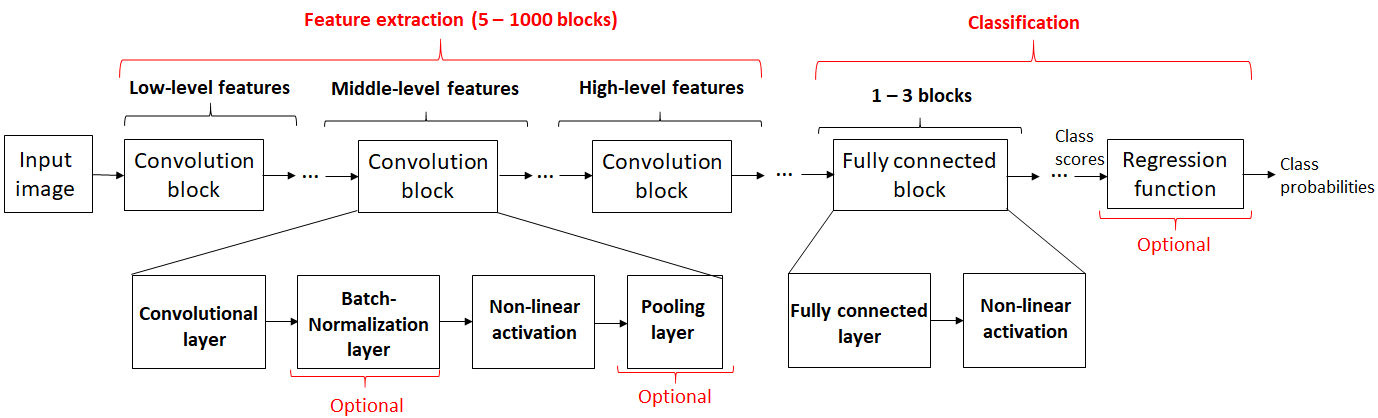
\includegraphics[width=\textwidth]{Figures/CNN.png}
  \caption{Constitution of a typical CNN.}
  \label{fig:CNN}
\end{figure}
\vspace{-6.5mm}

\subsection{Convolutional layer}

Convolutional layers perform 3D convolutions, which can be seen as a set of 2D convolutions. In 2D convolutions, a 2D kernel is overlapped and shifted as a sliding window throughout the entire 2D input image (known as input feature map), generating a 2D output image (called output feature map). In each overlap, a multiply and accumulate (MAC) operation is performed. Padding, which consists in adding new elements around the edges of the input feature map (FM), allows the output to keep the same size as the input. Normally zero-padding is applied. Fig.~\ref{fig:2D_conv} exemplifies a 2D convolution between an 5x5 input feature map and 3x3 kernel with zero padding. Note how the weights that compose the kernel are shared during the process. In this example, the step size (also known as stride) used when shifting the kernel throughout the input feature map is 1.   

\begin{figure}[!htb]
  \centering
  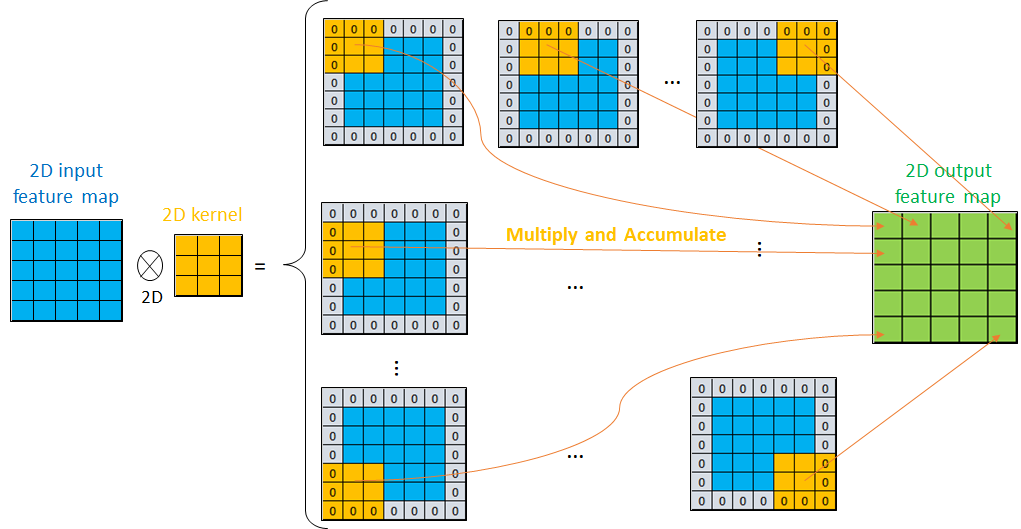
\includegraphics[width=0.9\textwidth]{Figures/2D_conv.png}
  \caption{Example of an 5x5 input feature map and 3x3 kernel 2D convolution.}
  \label{fig:2D_conv}
\end{figure}

The input of convolutional layers is a set of 2D feature maps (each one is called a channel) and another set of 3D kernels, with each 3D kernel having the same number of 2D channels. For each 3D kernel, there is a 2D convolution between each channel of the input feature map and each channel of the given 3D kernel. The results of the convolutions are summed across all the channels. The output feature map is obtained after summing the former result with a shared bias associated to each 3D kernel. Therefore, one output feature map is created for each 3D kernel. Fig.~\ref{fig:3D_conv} exemplifies a 3D convolution between an 5x5 input feature map and two 3x3 kernels, all with 3 channels and zero-padding.

\begin{figure}[!htb]
  \centering
  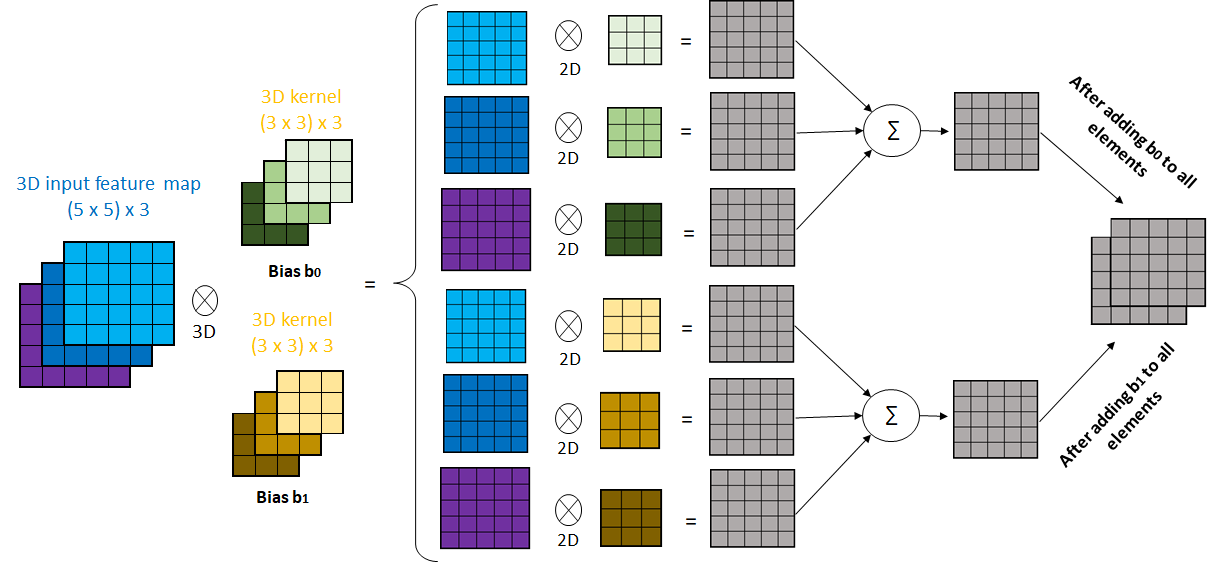
\includegraphics[width=\textwidth]{Figures/3D_conv.png}
  \caption{Example of an 5x5 input feature map and two 3x3 kernels 3D convolution (3 channels).}
  \label{fig:3D_conv}
\end{figure}
\vspace{-5mm}

\subsection{Batch-Normalization layer}

The batch-normalization layer is used for speeding up the training by normalizing the input data (i.e., zero mean and unit standard deviation)~\cite{Abdelouahab:dnn_survey}. Furthermore, the normalized value is scaled and shifted. Eq. \ref{eq:batch_norm} expresses the computation performed by this layer for each input element, $x$, where the mean, $\mu$, and the variance, $\sigma^2$, are statistics collected from training and the scale factor, $\gamma$, and the shift factor, $\beta$, are parameters learned during training. $\epsilon$ is a small constant that avoids dividing by zero. When using this layer, the bias can be included in the shift factor instead of being computed in the convolutional layer.

\begin{equation}
  y = \frac{x-\mu}{\sqrt{\sigma^2+\epsilon}} \gamma + \beta
\label{eq:batch_norm}
\end{equation}

In inference, the values of $\mu$, $\sigma^2$, $\gamma$ and $\beta$ are known. Thus, Eq. \ref{eq:batch_norm} can be reformulated as one multiplication and one addition, as shown in Eq. \ref{eq:batch_norm2}, where $\gamma_i$ and $\beta_i$ are the new scale and shift factors.

\begin{equation}
  y = x \times \frac{\gamma}{\sqrt{\sigma^2+\epsilon}} + \left( - \frac{\mu \times \gamma}{\sqrt{\sigma^2+\epsilon}} + \beta \right) = x \times \gamma_i + \beta_i
\label{eq:batch_norm2}
\end{equation}

\subsection{Pooling layer}

The pooling layer downsamples the feature maps, leading to a reduction of the number of parameters in the next layers. Each 2D channel is divided into non-overlapping blocks, which are further replaced by the maximum (max-pooling) or the mean (average pooling) value of the block. The most common operation is a 2x2 max-pooling, as shown in Fig.~\ref{fig:maxpool}. Some CNNs, instead of using pooling layers, simply apply a stride of 2 in the convolutional layers. However, pooling layers are more robust as they turn the network invariant to small shifts and distortions when downsampling~\cite{sze:dnn_survey}. 

\begin{figure}[!htb]
  \centering
  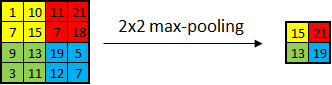
\includegraphics[width=0.45\textwidth]{Figures/maxpool.png}
  \caption{Example of 2x2 max-pooling.}
  \label{fig:maxpool}
\end{figure}
\vspace{-0.3cm}

\subsection{Shortcut layer}
The shortcut layer skips one or more layers by adding the output of a former layer to the input of the current layer. Fig.~\ref{fig:shortcut} exemplifies a shortcut layer generated from adding the output from 2 layers before.

\begin{figure}[!htb]
  \centering
  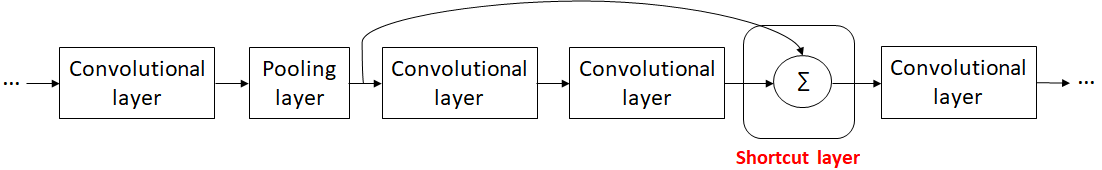
\includegraphics[width=0.85\textwidth]{Figures/shortcut_layer.png}
  \caption{Example of a shortcut layer.}
  \label{fig:shortcut}
\end{figure}
\vspace{-0.3cm}

\subsection{Route and upsample layers}

Route and upsample layers were introduced for CNNs focused on object detection tasks~\cite{Redmon2018YOLOv3AI}. The route layer concatenates the output from a former layer with the input of the current layer by stacking them into different channels. For example, routing a (26x26)x256 feature map with a (26x26)x128 feature map results in a (26x26)x384 feature map. This allows the detection of fine grained features, improving the localization of small objects. 

The upsample layer upsamples a feature map, typically by a factor of two, which allows to detect objects at different scales and obtain more meaningful semantic information from the features. Fig.~\ref{fig:upsample} exemplifies the simplest way to upsample a 2x2 feature map by a factor of two. 

\begin{figure}[!htb]
  \centering
  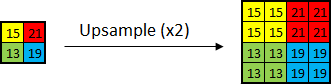
\includegraphics[width=0.45\textwidth]{Figures/upsample.png}
  \caption{Example of upsampling by a factor of 2.}
  \label{fig:upsample}
\end{figure}
\vspace{-0.4cm}

%%%%%%%%%%%%%%%%%%%%%%%%%%%%%%%%%%%%%%%%%%%%%%%%%%%%%%%%%%%%%%%%%%%%%%%%
\section{Training neural networks}
\label{section:training}

The training of neural networks consists in finding the parameters (i.e., weights and bias) that maximize the score of the correct prediction and minimize the scores of the incorrect predictions. For that, there is a training dataset containing inputs of the network (e.g., an image) and the desired output (e.g., label). In order to obtain the parameters, the gradient descent method~\cite{sze:dnn_survey} is used. This iterative algorithm updates the parameters by computing the partial derivatives of the gradient, which indicates how the parameters should change to reduce the difference between the desired outputs and the actual predictions (also known as loss). To efficiently compute the partial derivatives, the loss is propagated backwards through the network, which is known as the backpropagation algorithm~\cite{sze:dnn_survey}.  

Often, the parameters are initialized randomly for the first iteration of the gradient descent, which could result in slow training. To speed-up the training and achieve better performance, fine-tuning can be applied. Fine-tuning consists in using previously-trained parameters as a starting point to adjust the data to a new dataset or a new constraint.

There are several frameworks for training and testing DNN models. The most popular are Caffe, Tensorflow, Torch~\cite{sze:dnn_survey} and Darknet~\cite{Redmon2015YouOL}. The popular CNN models that will be mentioned in the next section were developed for image classification. The most popular datasets for this task are MNIST (digit classification), CIFAR and ImageNet~\cite{sze:dnn_survey}.

%%%%%%%%%%%%%%%%%%%%%%%%%%%%%%%%%%%%%%%%%%%%%%%%%%%%%%%%%%%%%%%%%%%%%%%%

\section{Popular CNN models}
\label{section:popular_models}

AlexNet~\cite{sze:dnn_survey} was one of the first CNN-based models for image classification, followed by VGG-16~\cite{sze:dnn_survey}. Both are based on the architecture presented in Fig.~\ref{fig:CNN}. They mainly differ in the number of layers and in the number and size of the kernels. A more distinct model is GoogLeNet~\cite{sze:dnn_survey}. Different sized filters are convoluted in parallel for the same input feature map and the results are further concatenated. Therefore, the input is processed at multiple scales. The other difference is the use of 1x1 kernels to reduce the number of channels and, consequently, the number of weights. 

ResNet~\cite{sze:dnn_survey} was the first CNN that exceeded the human-level accuracy for image classification by deploying a deeper network than the above-mentioned models. Those models suffered from the vanishing gradient problem, restraining them from getting deeper. When training, after several multiplications, the gradient becomes infinitely small during backpropagation, affecting the update of the weights in early layers for very deep networks. To avoid that, shortcut layers were added in the network.

Darknet-53~\cite{Redmon2018YOLOv3AI} is a more recent CNN model that also employs the shorcut layers first introduced by ResNet to allow a deeper network.  

%%%%%%%%%%%%%%%%%%%%%%%%%%%%%%%%%%%%%%%%%%%%%%%%%%%%%%%%%%%%%%%%%%%%%%%%
\section{FPGA-based CNNs}
\label{section:fpga_cnn}

Several studies have been conducted for accelerating CNNs in FPGAs~\citep{ma:loop_opt, sze:dnn_survey, Abdelouahab:dnn_survey, Guo:dnn_survey}. The main computation in CNNs is the MAC operation which mostly occurs in the convolutional layers, as shown in Table~\ref{tab:DNN}. Consequently, more than 90\% of the inference execution time is typically spent in the computation of the convolutional layers~\cite{Abdelouahab:dnn_survey}. Therefore, accelerators are focused on speeding-up these layers.

\vspace{+0.1cm}
\begin{table}[!htb]
    \footnotesize
    \centering
    \caption{Layer constitution of some popular DNN models (adapted from~\cite{Abdelouahab:dnn_survey}).}
    \label{tab:DNN}
    \begin{tabular}{|c|c|c|c|c|c|}
    \hline
            Type of layer              &  Characteristic & AlexNet &   VGG-16   &  GoogLeNet  &    ResNet-152  \\ \hline
   {\multirow{3}{*}{{Convolutional}}}  &     \# Layers   &    5    &    13     &      57     &     155    \\ \cline{2-6}
                                       &     \# MACs     &   666M  &   15.3G   &    1.58G    &    11.3G   \\ \cline{2-6} 
                                       &  \#Parameters   &  2.33M  &   14.7M   &    5.97M    &     58M    \\ \hline
              Pooling                  &      \# Layers   &    3    &    5     &      14     &      2     \\ \hline 
  {\multirow{3}{*}{{Fully Connected}}} &     \# Layers   &     3    &    3     &      1      &      1     \\ \cline{2-6}
                                       &     \# MACs     &   58.6M  &   124M   &    1.02M    &    2.05M   \\ \cline{2-6} 
                                       &  \#Parameters   &   58.6M  &   124M   &    1.02M    &    2.05M   \\ \hline
    \end{tabular}
\end{table}

The most common approaches for accelerating CNN inference in FPGAs in previous works are mainly focused on optimizing the accelerator by developing dedicated hardware and memory systems in order to exploit the parallelism of the MAC operations and to enhance data reuse. Approximating the model specifically for computation in FPGAs is another method that allows to reduce the amount of operations and storage requirements.

\subsection{Accelerator optimization}
\label{subsection:acc_opt}

One of the main advantages of accelerating CNNs in FPGAs, rather than in CPUs or GPUs, is the flexibility to design costumed hardware to exploit different sources of parallelism and dedicated caches to support data reuse. As shown in Table~\ref{tab:DNN}, as networks get deeper, the number of operations and the storage requirements increase. Consequently, the use of external memory is required, whose access results in high latency and significant energy consumption. FPGAs present a density of hard-wired Digital Signal Processing (DSP) blocks and a collection of on-chip memories that can be used for performing the MAC operations and reducing the number of external memory accesses, respectively.

Typical FPGA-based CNN accelerators~\cite{qiu:fpga_acc, zhang:fpga_acc, suda:fpga_acc} introduce several levels of memory hierarchy, as shown in Fig.~\ref{fig:fpga_cnn}. The system is composed by two on-chip input buffers, one for fetching the feature maps and the other for fetching the parameters (i.e., weights and bias) from the external memory through the DMA. The data is streamed into configurable processing elements (PEs), which are responsible for computing the MAC operations. Each PE has its own on-chip registers. The on-chip output buffer stores the intermediate results and output feature maps, which are transferred back, if needed, to the external memory. The CPU issues the workload to the controller, which in turn generates control signals to the other modules. The multipliers and adder trees present in each PE are usually pipelined in order to reduce the critical path of the circuit and increase the throughput.

\begin{figure}[!htb]
  \centering
  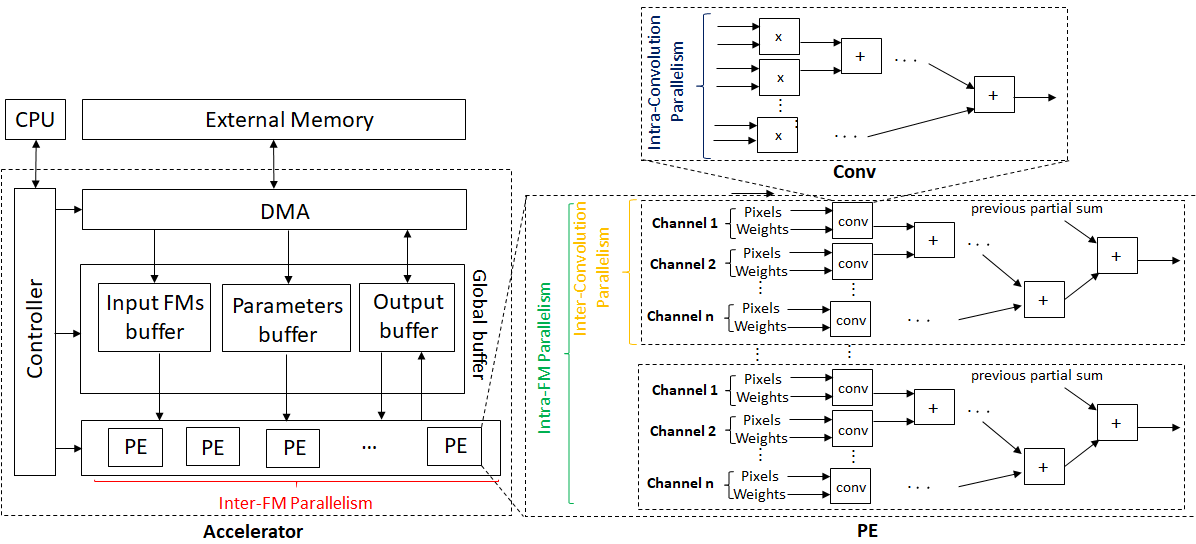
\includegraphics[width=\textwidth]{Figures/fpga_cnn.png}
  \caption{Typical FPGA-based CNN accelerator (adapted from~\cite{Abdelouahab:dnn_survey}).}
  \label{fig:fpga_cnn}
\end{figure}

Fig.~\ref{fig:fpga_cnn} also shows four sources of concurrency~\cite{Abdelouahab:dnn_survey} when computing each convolutional layer:\\
1) \underline{Intra-Convolution Parallelism:} multiplications in 2D convolutions are implemented concurrently.\\
2) \underline{Inter-Convolution Parallelism:} multiple 2D convolutions are computed concurrently.\\
3) \underline{Intra-FM Parallelism:} multiple pixels of a single output FM are processed concurrently.\\
4) \underline{Inter-FM Parallelism:} each output FM is processed separately in a different PE.

The computation of each convolutional layer can be seen as the application of four nested loops. Each loop is associated to a source of parallelism, as represented in Fig.~\ref{fig:loop_parall}.

\begin{figure}[!htb]
  \centering
  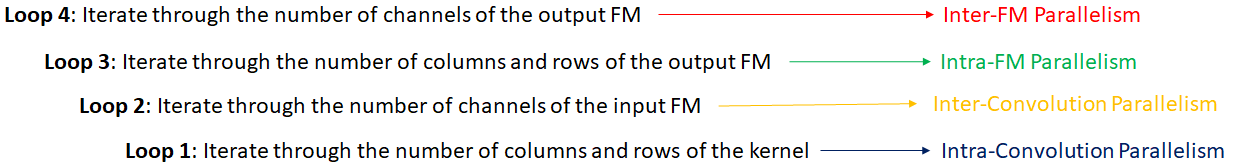
\includegraphics[width=\textwidth]{Figures/loop_parall.png}
  \caption{Association between loops and source of parallelism.}
  \label{fig:loop_parall}
\end{figure}

The sources of parallelism to be exploited depend on the characteristics of the convolutional layers (e.g., number of channels, input feature map size) and the FPGA resources. The architectural configuration of the PEs (i.e., number of MACs and registers) and the data temporal scheduling are defined by applying loop optimization techniques such as loop unrolling, loop tiling and loop interchange~\cite{Abdelouahab:dnn_survey}. Examples of previous works that implement these techniques are analyzed in section \ref{subsection:comparison_fpga_acc}.\\

\vspace{-0.5cm}

\textbf{Loop unrolling} consists in accelerating the execution of the loops at the expense of resource utilization. Each loop has an unroll factor that indicates how many times the respective loop is parallelized. Taking into account the loop enumeration in Fig.~\ref{fig:loop_parall}, the unroll factor for loop 4 determines the number of PEs while the unroll factors for the remaining loops determine the number of multipliers, adders and registers of each PE. The total number of multipliers is given by the product of the four unroll factors. The unroll factors must be carefully chosen, otherwise, they could lead to underutilization of the hardware. For instance, for any given loop, if the number of iterations is not divisible by the respective unrolling factor, then, the utilization ratio is less than 1~\cite{Guo:dnn_survey}. Fig.~\ref{fig:unroll_reuse} shows that the weights and the pixels can be reused by unrolling loops 3 and 4 respectively~\cite{ma:loop_opt}.

\vspace{-0.2cm}
\begin{figure}[!htb]
  \centering
  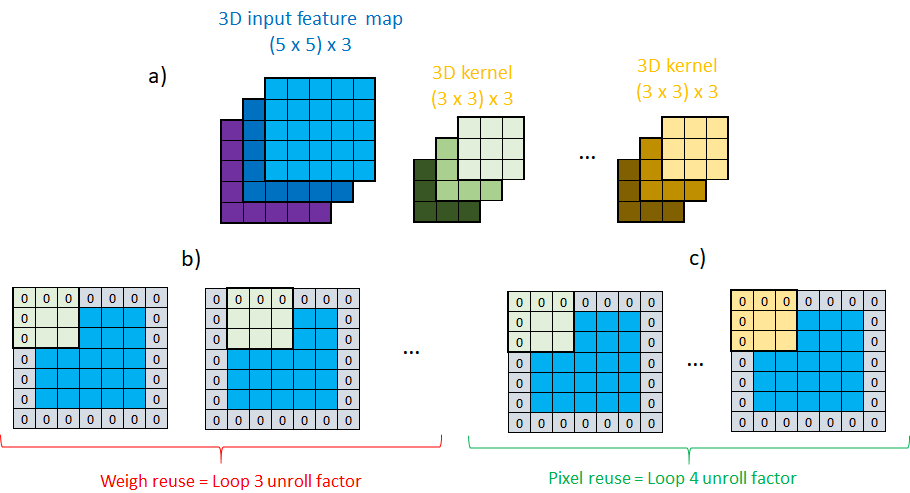
\includegraphics[width=0.85\textwidth]{Figures/unroll_reuse.png}
  \caption{a) 3D convolution between one FM and several kernels with b) weight and c) pixel reuse.}
  \label{fig:unroll_reuse}
\end{figure}

\textbf{Loop tiling} is a higher level of loop unrolling that divides the data into multiple blocks that fit into the on-chip buffers, increasing the data locality. Each tiled loop is splitted into two loops: one for iterating inside each tile (intra-tiling) and the other for iterating over the tiles (inter-tiling). Each loop has a tiling factor that indicates how many iterations are performed inside the respective tile. The tiling factors determine the size of the input and output buffers. If the tiling factors can cover all pixels and weights for loops 1 and 2, the partial sums (between channels) are stored in the local registers~\cite{ma:loop_opt}. Otherwise, the partial sums of one tile must be stored in the output buffer (intermediate result) until is used by the next tile~\cite{ma:loop_opt}. Fig.~\ref{fig:loop_tiling} exemplifies the division of the feature maps and kernels when tiling all loops.

\vspace{-0.2cm}
\begin{figure}[!htb]
  \centering
  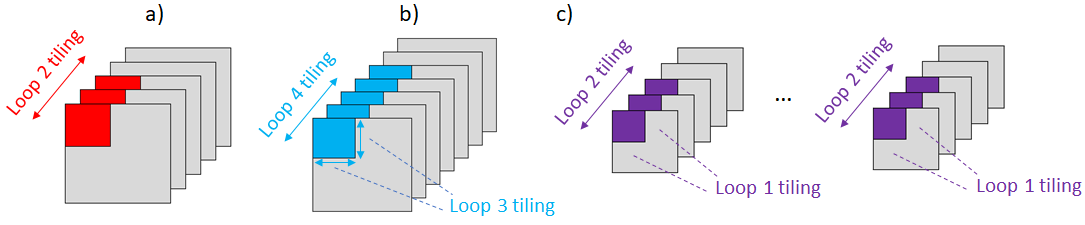
\includegraphics[width=0.85\textwidth]{Figures/loop_tiling.png}
  \caption{Example of loop tiling in the a) input FMs, b) output FMs and c) kernels.}
  \label{fig:loop_tiling}
\end{figure}
%\vspace{-0.5cm}

The \textbf{loop interchange} strategy decides the execution order of the loops. For intra-tiling loops, the order determines the data being transferred from the on-chip buffers to the PEs. For inter-tiling loops, the order indicates the movement of data from the external memory to the on-chip buffers. The storage required for intermediate results also depends on the order of the execution of the loops. For instance, the earlier loops 1 and 2 are computed, the fewer are the number of partial sums~\cite{ma:loop_opt}. 

\subsection{Model approximation}

The CNN execution can be accelerated by approximating the computation at the cost of minimal accuracy drop. Two of the most common strategies are reducing the precision and the number of operations. During training, the data is typically in single-precision floating-point format (32 bits). For inference in FPGAs, the feature maps and kernels can be converted to fixed-point format with less precision (typically 8 or 16 bits), reducing the storage requirements, hardware utilization and power consumption~\cite{Abdelouahab:dnn_survey}. 

The reduction of the FPGA resources consumption when using fixed-point representation is clear in Table~\ref{tab:resource_cons}, especially for lower precision data. The DSP consumption is hardly benefited when using narrower bit-width than 16 for fixed-point. Fig.~\ref{fig:fp_conv} exemplifies the conversion of a 32-bit floating-point value to fixed-point with 8 bits for the decimal part and 8 bits for the fractional part (Q8.8).

\vspace{+0.1cm}
\begin{table}[!htb]
    \footnotesize
    \centering
    \caption{Operation resource consumption for different operand sizes (adapted from~\cite{Guo:dnn_survey}).}
    \label{tab:resource_cons}
    \begin{tabular}{|c|c c|c c|c c c|}
    \hline
   \multirow{2}{*}{Data type} & \multicolumn{2}{|c|}{Multiplier} & \multicolumn{2}{|c|}{Adder} & \multicolumn{3}{|c|}{Multiplier and Adder} \\ \cline{2-8}
                              & LUT & FF & LUT & FF & LUT & FF & DSP \\ \hline
   floating-point (32 bits)   & 708 & 858 & 430 & 749 & 800 & 1284 & 2 \\ \hline
   floating-point (16 bits)   & 221 & 303 & 211 & 337 & 451 & 686 & 1 \\ \hline
   fixed-point (32 bits)      & 1112 & 1143 & 32 & 32 & 111 & 64 & 4  \\ \hline
   fixed-point (16 bits)      & 289 & 301 & 16 & 16 & 0 & 0 & 1  \\ \hline
   fixed-point (8 bits)       & 75 & 80 & 8 & 8 & 0 & 0 & 1  \\ \hline
   fixed-point (4 bits)       & 17 & 20 & 4 & 4 & 0 & 0 & 1  \\ \hline
    \end{tabular}
\end{table}

\vspace{-0.5cm}
\begin{figure}[!htb]
  \centering
  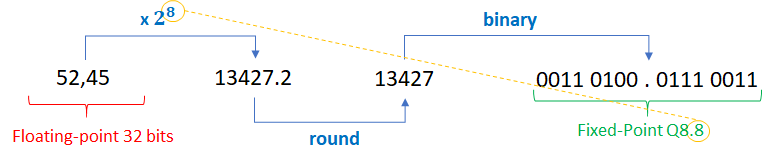
\includegraphics[width=0.7\textwidth]{Figures/fp_conv.png}
  \caption{Example of conversion from 32 bits floating-point to Q8.8 fixed-point.}
  \label{fig:fp_conv}
\end{figure}

In general, the feature maps of deeper layers tend to present a larger numerical range than the ones from initial layers and the weights also tend to be much smaller than the feature maps~\cite{Guo:dnn_survey}. Moreover, to prevent overflow, the precision must be increased for intermediate results. Thus, different precision values are normally used for weights, intermediate results and output feature maps from different layers. 

In order to reduce the number of operations, the most common approaches are weight pruning and low rank approximation~\cite{Abdelouahab:dnn_survey}. These methods are often followed by a fine-tuning phase to counterbalance the accuracy drop. As this work is focused on the inference part, these methods are not further studied.

\subsection{Comparison of FPGA-based CNN accelerators}
\label{subsection:comparison_fpga_acc}

To choose the unroll and tiling factors that maximize both computational throughput and resource utilization, besides minimizing the number of memory accesses, previous works performed a brute force exploration of the design space~\cite{Abdelouahab:dnn_survey}. This design space exploration consists in testing several factors for different loops in order to exploit various parallelism and data reuse patterns.

~\cite{zhang:fpga_acc} was one of the first works to employ loop optimization strategies to accelerate the execution of AlexNet in a FPGA. By unrolling loops 2 and 4, the accelerator achieved a computational throughput of 61.62 GOPs, relying on 32-bit floating point arithmetic. This work also introduced the utilization of double buffers to perform ping-pong operations, allowing to simultaneously compute and transfer data.

Greater acceleration can be achieved when using loop optimization techniques alongside fixed-point arithmetic. For instance,~\cite{suda:fpga_acc} reached a computational throughput of 187.24 GOPs for the same AlexNet network by unrolling loops 1, 2 and 4, relying on 16-bit fixed-point arithmetic. In general, unrolling loop 1 does not provide enough parallelism as the kernels are usually small (e.g. 3x3). Unrolling loop 1 also increases control complexity when layers present different kernel sizes. 
 
The same unrolling scheme and fixed point arithmetic was followed by~\cite{qiu:fpga_acc} for the VGG-16 network, achieving a throughput of 136.97 GOPs. In all these approaches, the loops are unrolled in the same way they are tilled~\cite{Abdelouahab:dnn_survey}. In~\cite{ma:loop_opt}, the tiling factors are set in a way all the data required to compute an element from the output feature map is fully buffered. As a result, intermediate results can be stored in the PE registers instead of in the output buffer. This accelerator outperforms all previous implementations by reusing pixels and weights when unrolling loops 3 and 4, reaching a total throughput of 645.25 GOPs.  

Table~\ref{tab:comp_fpga_acc} compares the four FPGA-based accelerators in terms of resource consumption, optimization strategy and throughput. All these approaches unroll loop 4 by employing several PEs.~\cite{zhang:fpga_acc} has the major DSP consumption mainly due to using 32-bit floating point operands.~\cite{ma:loop_opt} presents 3 times higher throughput than~\cite{qiu:fpga_acc} but consumes the double of resources in terms of DSPs and on-chip memory (BRAMs). The analysis of previous works regarding FPGA-based CNN acceleration allows to infer that a design exploration is essential for achieving optimal unroll and tiling factors, which in turn depend on the characteristics of the convolutional layers and the available resources of the FPGA. 

\vspace{+0.1cm}
\begin{table}[!htb]
    \footnotesize
    \centering
    \caption{Comparison between different FPGA-based accelerators.}
    \label{tab:comp_fpga_acc}
    \begin{tabular}{|>{\columncolor[gray]{0.8}}c|c|c|c|c|}
    \hline
    Network & AlexNet~\cite{zhang:fpga_acc} & AlexNet~\cite{suda:fpga_acc} & VGG-16~\cite{qiu:fpga_acc} & VGG-16~\cite{ma:loop_opt} \\ \hline
    Device & Virtex VX485T & Stratix5 GSD8 & Zynq XC7Z045 & Arria-10 GX 1150  \\ \hline
    Frequency (MHz) & 100 & 120 & 150 & 150 \\ \hline
    \# Operations (GOP) & 1.3 & 1.3 & 30.76 & 30.95\\ \hline
    \# Weights (M) & 2.3 & 2.3 & 50.18 & 138.3\\ \hline
    LUT (K) & 186 & 138 & 183 & 161\\ \hline
    BRAM & 512 (36 kB) & --- &  486 (36 kB) & 1900 (20 kB) \\ \hline
    DSP & 2240 & 635 & 780 & 1518 \\ \hline
    Throughput (GOPs) & 61.62 & 126.6 & 136.97 & 645.25 \\ \hline
    Unrolled loops & 2,4 & 1,2,4 & 1,2,4 & 3,4 \\ \hline
    Precision & Float 32 & Fixed 16 & Fixed 16 & Fixed 8-16\\ \hline
    \end{tabular}
\end{table}

\subsubsection{Final remarks}

CNNs are composed by a sequence of interconnected layers, being the convolutional ones the most time consuming for inference execution. FPGAs, with dedicated hardware and cache memories, allows to exploit parallelism and data reuse. Previous works use fixed-point arithmetic and perform design space exploration to obtain the best loop optimization parameters. A similar study will need to be conducted to accelerate the convolutional layers of the object detection network chosen in the next chapter.